\documentclass[tikz,border=3pt]{standalone}
\usepackage{fontspec}
\usepackage{amsmath}
\usepackage{xcolor}
\usepackage{tikz}
\usepackage{pgfplots}
\pgfplotsset{compat=1.18}
\usetikzlibrary{arrows.meta,calc,fit,positioning,shapes.geometric,shapes.misc,patterns,plotmarks}
\IfFontExistsTF{Arial}{\setsansfont{Arial}}{\setsansfont{TeX Gyre Heros}}
\renewcommand{\familydefault}{\sfdefault}
\tikzset{
  >={Stealth[length=2.2mm,width=1.5mm]},
  exact title/.style={font=\bfseries\fontsize{10.5}{12}\selectfont,align=center},
  exact subtitle/.style={font=\fontsize{6.3}{7.2}\selectfont,align=center},
  exact label/.style={font=\fontsize{6.4}{7.5}\selectfont,align=center},
  exact tiny/.style={font=\fontsize{5.3}{6.3}\selectfont,align=center},
  panel/.style={draw=black!14,rounded corners=1.2mm,fill=white,line width=.45pt},
  neutral/.style={draw=black!30,fill=black!3,rounded corners=1mm,line width=.45pt},
  arrow/.style={-Stealth,line width=.7pt},
  softarrow/.style={-Stealth,line width=.55pt,draw=black!45},
  dashedarrow/.style={-Stealth,dashed,line width=.55pt,draw=black!55},
  metric/.style={font=\fontsize{5.3}{6.3}\selectfont,fill=white,inner sep=1pt},
}
\newcommand{\pill}[4]{\node[draw=#2!70,fill=#2!10,rounded corners=1.5mm,inner xsep=3pt,inner ysep=2pt,exact label,text=#2] (#1) at #3 {#4};}
\newcommand{\frameboxx}[4]{\draw[draw=#2!65,fill=#2!8,rounded corners=.6mm,line width=.5pt] (#1.south west) rectangle (#1.north east);\node[exact tiny,text=#2] at #3 {#4};}
\newcommand{\axislabel}[3]{\node[exact tiny,text=black!60] at (#1) {#2};\node[exact tiny,text=black!60,rotate=90] at (#3) {#2};}

\definecolor{usblue}{HTML}{4C78A8}\definecolor{usorange}{HTML}{F58518}\definecolor{usgray}{HTML}{A0A6AD}\definecolor{usink}{HTML}{263238}
\begin{document}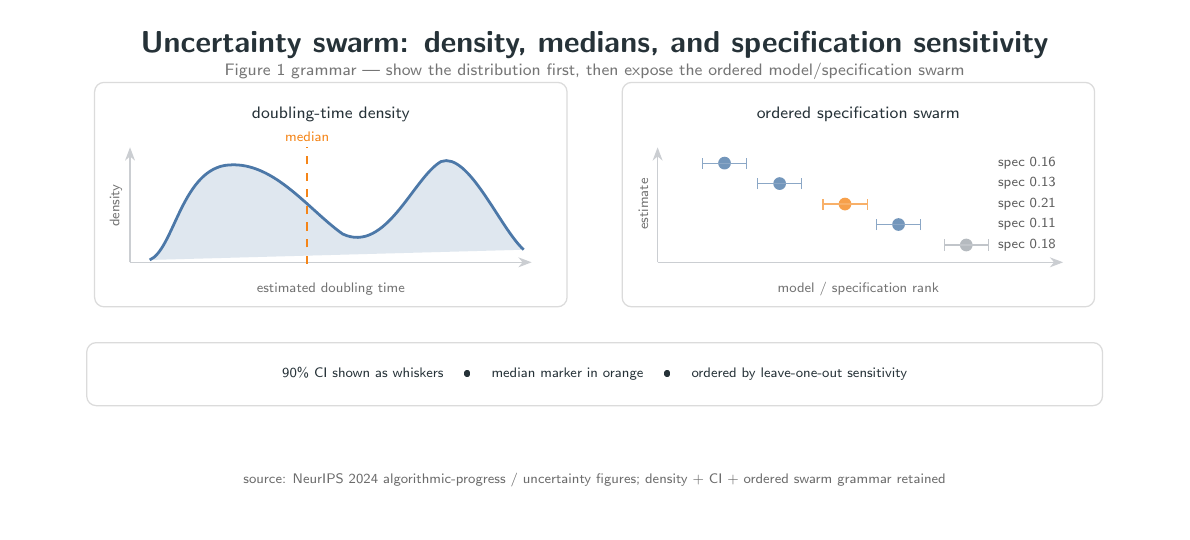
\begin{tikzpicture}[x=1cm,y=1cm]
\path[use as bounding box] (-.2,-3.95) rectangle (14.2,2.2);
\node[exact title,text=usink] at (7,1.98) {Uncertainty swarm: density, medians, and specification sensitivity};
\node[exact subtitle,text=black!54] at (7,1.64) {Figure 1 grammar — show the distribution first, then expose the ordered model/specification swarm};
\node[panel,minimum width=6.0cm,minimum height=2.85cm] at (3.65,.08) {};
\node[panel,minimum width=6.0cm,minimum height=2.85cm] at (10.35,.08) {};
\node[exact label,text=usink] at (3.65,1.1) {doubling-time density};\draw[usgray!55,-Stealth] (1.1,-.78) -- (6.2,-.78);\draw[usgray!55,-Stealth] (1.1,-.78) -- (1.1,.68);\fill[usblue!18] (1.35,-.75) .. controls (1.65,-.62) and (1.75,.35) .. (2.3,.45) .. controls (2.9,.54) and (3.35,-.1) .. (3.8,-.42) .. controls (4.35,-.68) and (4.7,.3) .. (5.05,.5) .. controls (5.4,.63) and (5.8,-.35) .. (6.1,-.62) -- cycle;\draw[usblue,line width=1pt] (1.35,-.75) .. controls (1.65,-.62) and (1.75,.35) .. (2.3,.45) .. controls (2.9,.54) and (3.35,-.1) .. (3.8,-.42) .. controls (4.35,-.68) and (4.7,.3) .. (5.05,.5) .. controls (5.4,.63) and (5.8,-.35) .. (6.1,-.62);\draw[usorange,dashed,line width=.9pt] (3.35,-.8) -- (3.35,.68);\node[exact tiny,text=usorange] at (3.35,.82) {median};\node[exact tiny,text=black!55] at (3.65,-1.12) {estimated doubling time};\node[exact tiny,text=black!55,rotate=90] at (.92,-.06) {density};
\node[exact label,text=usink] at (10.35,1.1) {ordered specification swarm};\draw[usgray!55,-Stealth] (7.8,-.78) -- (12.95,-.78);\draw[usgray!55,-Stealth] (7.8,-.78) -- (7.8,.68);\foreach \y/\x/\c/\ci in {.48/8.65/usblue/0.16,.22/9.35/usblue/0.13,-.04/10.18/usorange/0.21,-.3/10.86/usblue/0.11,-.56/11.72/usgray/0.18}{\fill[\c!78] (\x,\y) circle (2.3pt);\draw[\c!65] (\x-.28,\y) -- (\x+.28,\y);\draw[\c!65] (\x-.28,\y-.07) -- (\x-.28,\y+.07);\draw[\c!65] (\x+.28,\y-.07) -- (\x+.28,\y+.07);\node[exact tiny,text=black!63,anchor=west] at (12.0,\y) {spec \ci};}\node[exact tiny,text=black!55] at (10.35,-1.12) {model / specification rank};\node[exact tiny,text=black!55,rotate=90] at (7.62,-.04) {estimate};
\node[panel,minimum width=12.9cm,minimum height=.8cm] at (7,-2.2) {};\node[exact tiny,text=usink] at (7,-2.2) {90\% CI shown as whiskers \quad • \quad median marker in orange \quad • \quad ordered by leave-one-out sensitivity};
\node[exact tiny,text=black!58] at (7,-3.55) {source: NeurIPS 2024 algorithmic-progress / uncertainty figures; density + CI + ordered swarm grammar retained};
\end{tikzpicture}\end{document}
